\chapter{O projeto do produto}
\label{chap:projeto_do_produto}

Existem diversos tipos de projetos necessários à implementação e funcionamento de uma empresa industrial. O presente capítulo foca no projeto do produto, que é uma atividade complexa e subdividida em diversas etapas: geração do conceito, triagem do conceito, projeto preliminar, avaliação do projeto preliminar, construção de protótipos e projeto final do produto.  O projeto final do produto tem como resultados entregáveis o conceito final, o pacote de documentos e a descrição de processos. O fluxograma mostrado na Figura \ref{fig:projeto_produto} apresenta, em linhas gerais, as etapas presentes neste processo, mesmo que, na prática os projetistas avancem ou retrocedam pelas etapas de forma iterativa. Serão descritas a seguir cada etapa deste processo na ordem em que geralmente ocorrem.

\begin{figure}[H]
  \centering
  \caption{Fluxograma das etapas do projeto do produto.}
  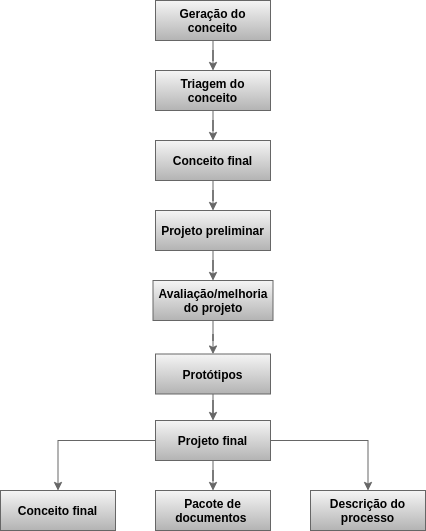
\includegraphics[width=.7\textwidth]{images/projeto_produto.png}
  \caption*{Fonte: Adaptado \cite{slack2006administracao} }
  \label{fig:projeto_produto}
\end{figure}

%! aqui esta sendo feita uma itemização diferente da feita no capítulo anterior
\textbf{Geração do conceito:} É a primeira etapa para o desenvolvimento do projeto de um produto. É nesta fase que se elabora um resumo completo do conjunto de benefícios que o produto, quando fabricado, deverá proporcionar ao seu usuário, podendo este ser ou não cliente direto da empresa. Tais benefícios devem corresponder às necessidades, desejos e expectativa do usuário, portanto, esta é uma atividade sob responsabilidade da equipe de \textit{marketing}, pois são eles que fazem a ponte entre o usuário e a equipe operacional da empresa.

\textbf{Triagem do conceito:} Nesta etapa ocorre uma avaliação entre as diversas alternativas de conceitos concebidas na etapa anterior. Esta avaliação, segundo \cite{slack2006administracao}, deve considerar a importância de cada solução proposta, de modo que possam ser feitas escolhas entre elas. Cada opção é avaliada a partir de três categorias de critérios: a viabilidade - ``Quão difícil é o projeto?'', a aceitabilidade - ``O projeto vale a pena?'' e a vulnerabilidade - ``O que pode dar errado?''.

\textbf{Conceito final:} Concluídas as avaliações da etapa anterior, obtém-se um conceito final do produto, que servirá de base para toda a parte de detalhamento técnico: forma, design, materiais, funcionalidades, resistência, segurança, durabilidade em uso e disponibilidade após a vida útil do produto. É importante lembrar que nesta etapa, ainda, não é apresentado os detalhes técnicos do produto, mas é indispensável para o referido detalhamento.

\textbf{Projeto preliminar:} Nesta etapa se inicia o detalhamento das informações de natureza técnica, fundamentais para a concepção do produto. Os documentos gerados nesta fase são, a princípio, os mesmos que farão parte da documentação final do projeto.

\textbf{Avaliação/melhoria do projeto:} O projeto do produto é uma atividade interativa, ou seja, está sujeita a sucessivas otimizações a medida em que evolui. Existem diversas técnicas ou ferramentas para a revisão e melhoria do projeto de um produto, dentre elas, destacam-se: o \ac{QFD}, engenharia de valor e os testes acelerados de resistência.

\textbf{Protótipos:} Antes da empresa colocar seu produto em produção regular, ela constrói exemplares iniciais do seu produto. O objetivo desta etapa é realizar testes e ensaios para observar o desempenho do protótipo em relação aos conceitos e projetos em fase de avaliações e melhorias.

\textbf{Projeto final:} A última etapa do processo consiste em elaborar um documento que contenha o conjunto de informações e especificações técnicas, que não deixem margem à dúvidas ou equívocos, para a produção do produto para o mercado. Segundo \cite{slack2006administracao}, a documentação final do projeto de um produto deve conter: o conceito final definitivo, ``pacote de documentos do produto'' (estrutura do produto, lista de materiais, especificações técnicas e seus componentes) e a descrição do processo de fabricação/montagem do produto (fluxograma).


\section{Aplicação Prática}
\label{sec:projeto_do_produto_aplicacao}

De certa forma, uma vez que o produto da SunBurn é energia elétrica, que deve ser entregue de forma estabelecida pelas instruções normativas da \ac{ANEEL} e de acordo com as características adotadas pelas linhas de transmissão aonde a unidade produtiva será instalada, o projeto de produto se dá apenas na adequação das características de tensão, forma de onda e frequência da energia produzida. Assim, o conceito final do produto pode ser caracterizado como energia elétrica com certo nível de tensão na faixa de kV e onda senoidal com frequência de 60 Hz.

A descrição do processo de fabricação deste produto foi realizada no Capítulo \ref{chap:tipos_de_processo_de_producao}, haja visto que o mesmo é fábricado de forma contínua. Em linhas gerais, a energia solar é transformada em energia elétrica com corrente contínua e baixa tensão pelos painéis fotovoltaicos. Em seguida a mesma é convertida para energia elétrica com corrente alternada pelos inversores, com subsequente elevação das tensões nos transformadores para o nível das linhas de transmissão.

Não foi possível o acesso ao pacote de documentos do processo de fabricação da SunBurn.